\documentclass{article}

\usepackage{graphicx}

\newcommand{\twopartdef}[4]
{
    \left\{
    \begin{array}{ll}
        #1 & #2 \\
        #3 & #4
    \end{array}
    \right.
}

\newcommand{\threepartdef}[6]
{
    \left\{
    \begin{array}{ll}
        #1 & #2 \\
        #3 & #4 \\
        #5 & #6
    \end{array}
    \right.
}

\begin{document}

\title{Time Range Queries for Hereditary Properties \\ \large 6.854 Final Project}
\author{Arsen Mamikonyan, Hayk Saribekyan}

\maketitle

\begin{abstract}
    Time range queries are important for analysing large datasets with timestamps. Such datasets are common in computational geometry, where a sequence of points with timestamps often corresponds to a trajectory of an object. Time range queries in this case check a certain property of section of the trajectory.
    
    In this paper we review recent general frameworks that can be used to handle property testing queries for time ranges, and discuss their implementations for solving certain problems in computational geometry. The results are limited to \textit{hereditary} properties, which cover a large variety of interesting problems.
    
    For two different hereditary properties, we compared the performance of efficient an algorithm and a naive one in practice. We observed that the efficient algorithms require more than ten times the amount of code in certain cases, but the large constant factor associated with it is compensated when working with large datasets.
\end{abstract}

\section{Introduction}
\label{sec:intro}
With the abundance of GPS and other movement tracking sensors there is a large amount of timestamped location data. The movement of an object in space can be modelled by a sequence of points $S = s_1, \dots, s_n$. To analyse the trajectory of the movement, one may want to check a certain property $P$ for portions $S[i, j] = s_i, \dots, s_j$ of $S$ for given values of $i$ and $j$. This paper discusses how to efficiently address such queries when $P$ satisfies the following two properties:
\begin{itemize}
    \item $P$ is boolean.
    \item $P$ is hereditary. This means that for a given sequence $S$, if $P(S)$ is true, then $P(S')$ is true for any continuous subsequence $S'$ of $S$.
\end{itemize}

In this paper we discuss and implement two properties for a sequence of points $S = s_1, \dots, s_n$:
\begin{itemize}
    \item \textit{Monotonicity}:  $S$ is \textit{monotone} if there is a direction vector $v$ such that TODO. In terms of trajectories, monotonicity shows whether the object travelled more or less in the same direction.
    
    \item \textit{Closeness}: $S$ is \textit{close} if any pair of points in $S$ is at most of distance $1$. One could use closeness queries to detect if a moving object mostly stayed in the same surrounding.
\end{itemize}

For a property $P$ satisfying the restrictions above, let $j^*(i)$ be the largest index $j$ such that $P$ holds for $S[i, j^*(i)] = s_i, \dots, s_{j^*(i)}$. Now notice, that since $P$ is a hereditary property $P(S[i, j]) = true$ if and only if $j \leq j^*(i)$. Therefore, if we construct $j^*(i)$ we can answer property testing queries in $O(1)$. Therefore, for the rest of the paper our goal will be to efficiently compute $j^*(i)$.

Bokal et al. \cite{bokal2015} propose an algorithms that compute $j^*(i)$ in $O(n)$ time for monotonicity, and in $O(n\log^2 n)$ time for closeness. Chan and Pratt \cite{chan2016} describe a different algorithm to achieve the same result for closeness, but also improve it to $O(n\log n)$ using fractional cascading.

The rest of the paper is organized as follows: Section \ref{sec:naive} describes the naive algorithms we developed to solve the problems we selected; in Section \ref{sec:monotonicity} we review the general framework that is set in \cite{bokal2015} for solving time range query problems, and show how it is applied to computer $j^*(i)$ for monotonicity. Section \ref{sec:closeness} reviews the framework by \cite{chan2016} and its application for the closeness property. We then give some implementation details in Section \cite{sec:implementation}, and describe the experimental setup and our tests in Section \cite{sec:experiments}.

\section{Naive Algorithms}
\label{sec:naive}
Suppose that for a sequence of length $n$ a property $P$ can be checked in $T_P(n)$ time. Then, one can compute $j^*(i)$ using binary search for each $i$. On a step of a binary search concerning a range $[l, r]$ the algorithm would spend $T_P(r - l)$ time. The total runtime of this simple algorithm is $O(nT_P(n)\log n)$. Call this algorithm $SN$ (stands for super-naive). For the problems of monotonicity and closeness we can do better.

\subsection{Monotonicity}
To detect whether a sequence is monotone or no, we can process the points while keeping a set of polar angles (field-of-view or FoV) that a direction vector $v$ can have. Notice that the FoV is always an interval. When a new point arrives we can update the FoV in constant time. If the FoV ever becomes empty, then the given sequence is not monotone. This algorithm runs in $O(n)$ time for a sequence of length $n$. Using this submodule for $SN$ we would get a $O(n^2\log n)$ algorithm.

However, doing a binary search for monotonicity is redundant, since we will do the same computation many times. Instead, for each $i$ proceed with the FoV computation until it is empty, which will happen precisely when we reach $j^*(i) + 1$. The resulting algorithm runs in $O(n^2)$ time.

\subsection{Closeness}
The simple method of closeness-check takes $O(n^2)$ for a sequence of $n$ points, because one has to check all pairs of points. This results in $SN$ runtime of $O(n^3\log n)$, which is super-slow. We can improve the closeness-check to $O(n\log n)$ using furthest-point Voronoi diagrams, but that would not qualify for $SN$ and would also take $O(n^2 \log^2 n)$ time to compute, which is also not fast.

Define $k*(i)$ as the largest index such that $d(s_i, s_j) \leq 1$ for all $j \leq k*(i)$. Clearly, $k^*(i) \geq j^*(i)$. Also, notice that $k^*$ can be computed in $O(n^2)$ for all points.

\textbf{Claim TODO - formatting} For $i < n$ $j^*(i) = \min( j^*(i + 1), k^*(i) )$

\textbf{Proof} obvious (should we even prove this?

This claim gives us an $O(n^2)$ $SN$ construction of $j^*(i)$ for the closeness property.

\section{something and Monotonicity TODO}
\label{sec:monotonicity}
Bokal et al. introduced an elegant framework to deal with range queries for hereditary problems. The key idea in their work is to greedily split the given set of points into ranges, defined by anchor points, and solve for each using a divide and conquer. To simplify the reasoning we first define a property matrix $A_P$ such that
\[ A_P(i, j) = \twopartdef{1}{P(S[i, j]) = true}{0}{P(S[i, j]) = false} \]

Suppose that there is an algorithm $J_P$ that, for a given $i$, finds $j^*(i)$ (notice that even if such $J_P$ exists, we are not happy to run it $n$ times for each $i$). We use $J_P$ to find \textit{anchor} points in $S$ as follows. Let $a_k$ be the index of $k^{th}$ anchor point in $S$. We define $a_1 = s_1$, $a_k = j^*(a_{k-1})$ for $k > 1$. Thus, the anchor points can be found using $J_P$. Figure \ref{fig:property_matrix} TODO shows the anchor points on $A$.

\begin{figure}
    \centering
    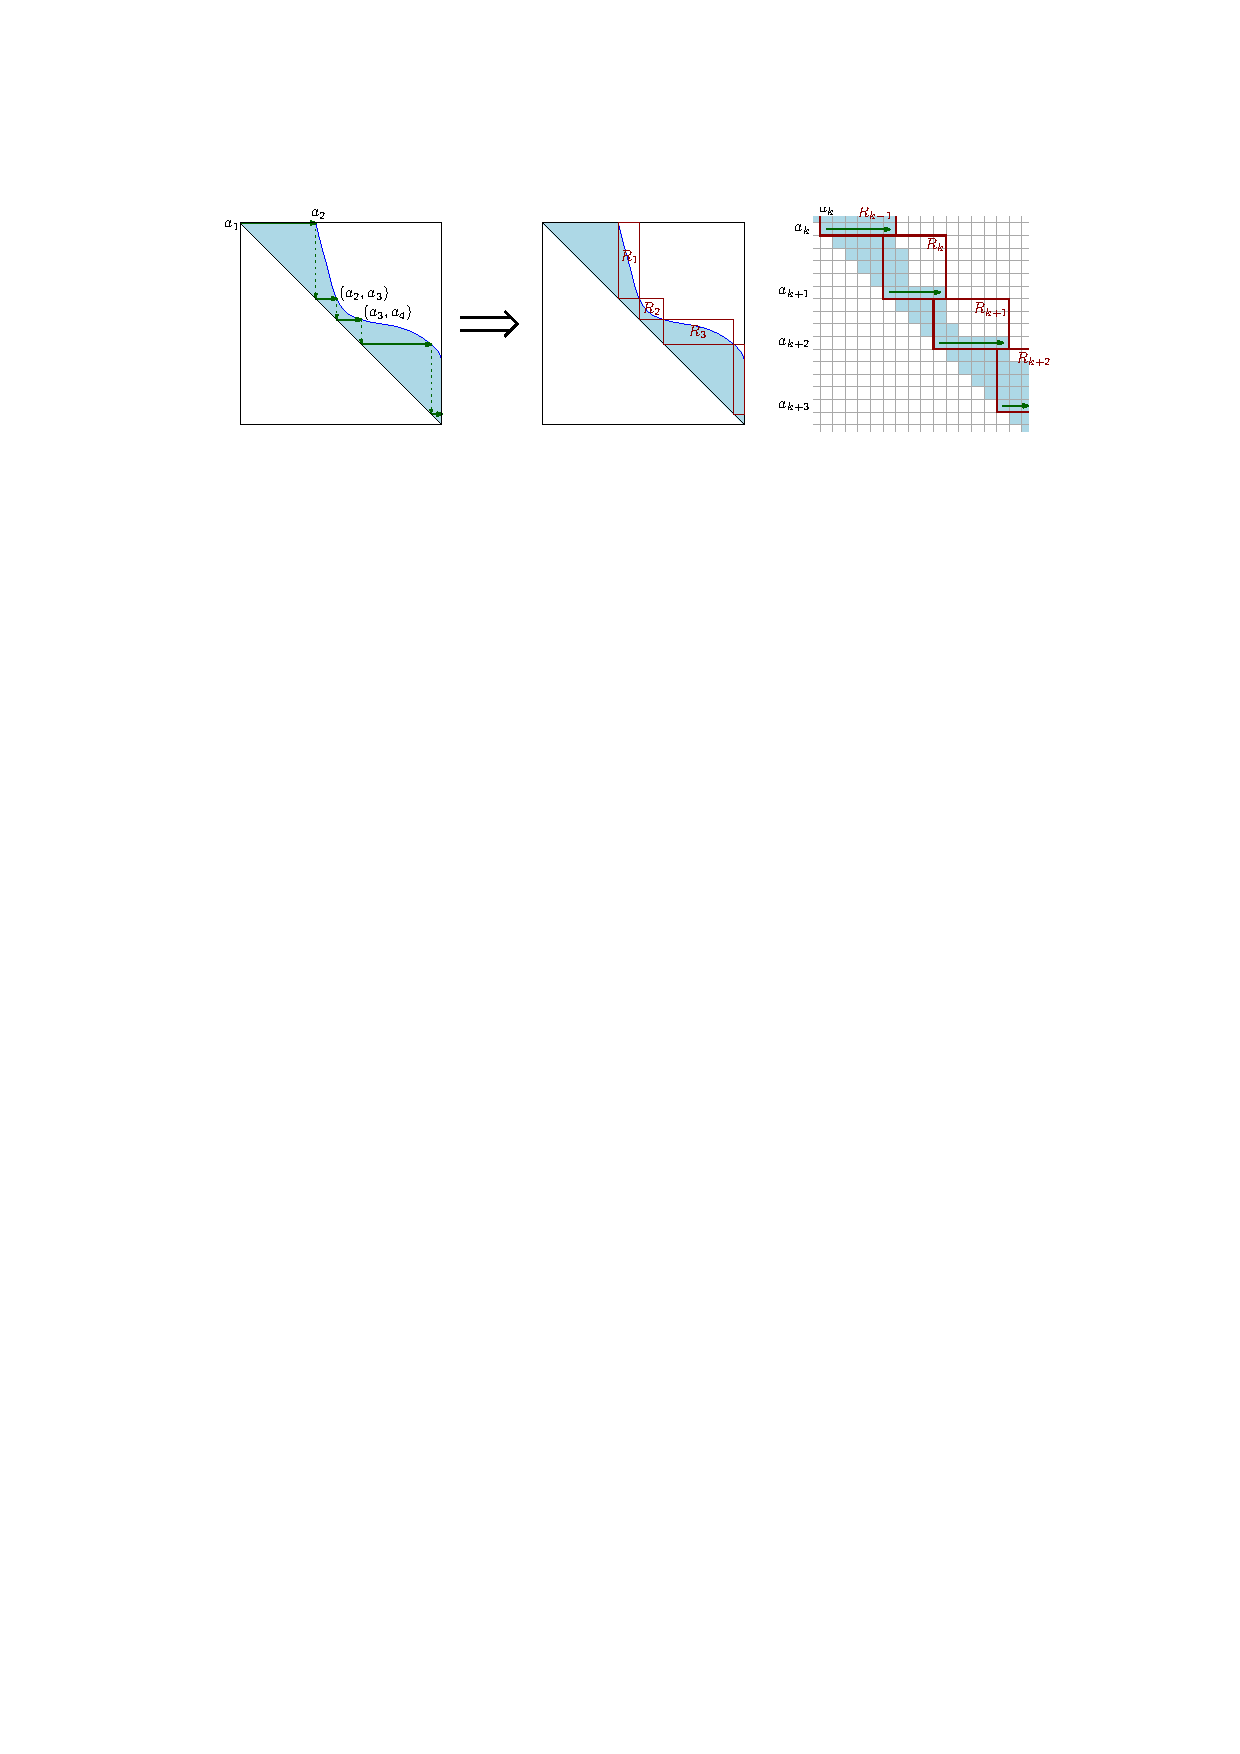
\includegraphics[width=1.2\textwidth]{figures/property_matrix.pdf}
    \label{fig:property_matrix}
    \caption{property matrix}
\end{figure}

As shown in Figure \ref{fig:property_matrix} the anchor points form rectangles. If we find the frontier (the curve in $A$ separating 1's from 0's) for each rectangle, then we are done. 

\section{something and Closeness TODO}
\label{sec:closeness}

\section{Implementation Details}
\label{sec:implementation}
- decided to implement chan's algorithm because the other one had voronoi and persistent data structure (or something similar) for point location in voronoi

- chan's algorithm is closer to what we've done in class (envelopes)

\section{Experiments}
\label{sec:experiments}
- mention that we have used random walk to mimic reality. in that case the good algorithm for monotonicity is not that good. but for the worst case, it's great.

- 

\section{Conclusion}
\label{sec:conclusion}

We will describe their algorithm for monotonicity property, which due to its simplicity does not require a divide and conquer in the second stage of the algorithm.

\section{Our contribution}
We've implemented
\begin{itemize}
\item In $O(n)$ time  we  can  find  all  maximal  subsequences  that  define  monotone  paths  in  some (subpath-dependent) direction. \cite{bokal_et_al:LIPIcs:2015:5113} 
\item In $O(n \log^2 n)$ time time we can find all maximal subsequences with diameter at most 1. \cite{chan_et_al:LIPIcs:2016:5920}
\end{itemize}

\section{Algorithms}
\subsection{$k^*$}

Let $k^*(i) = \inf_{m \geq i} \{d(i, m) > 1\}$. \textbf{Claim} $j^*(i-1) = \min(j^*(i), k^*(i-1))$. Thus after we calculate $k^*(i)$ for all elements, we can calculate $j^*(i)$ in $O(n)$ time by looping over all indices in the reverse order.

\subsection{Bokal et al Overview}
TODO: A page that deftly describes the algorithm we've implemented.

\subsection{Chan, Prat Overview}
TODO: A page that deftly describes the algorithm we've implemented.

\section{Implementation Details}
In this section we discuss some implementation details of the Chan, Pratt algorithm for diameter query problem. We skip the details of the monotonicity query, because it was relatively simple.

The novelty of the algorithm from Chan, Pratt is how they combine 1D range tree, with secondary structure that stores circle intersections. While the algorithm is elegant, its implementation is not. In particular, it is necessary to implement an intersection algorithm for arbitrary \textit{polyarcs}. A polyarc is a convex object, similar to a polygon, but instead of straight edges each side is an arc of a circle. The algorithm for the intersection of polyarcs is similar to that of polygons, however there are many more edge cases to consider.

\section{Experimental Results}

\subsection{Monotonicity}

TODO: Describe Naive algorithm which is a $O(n^2)$ algorithm.

\begin{figure}[!ht]
  \centering
  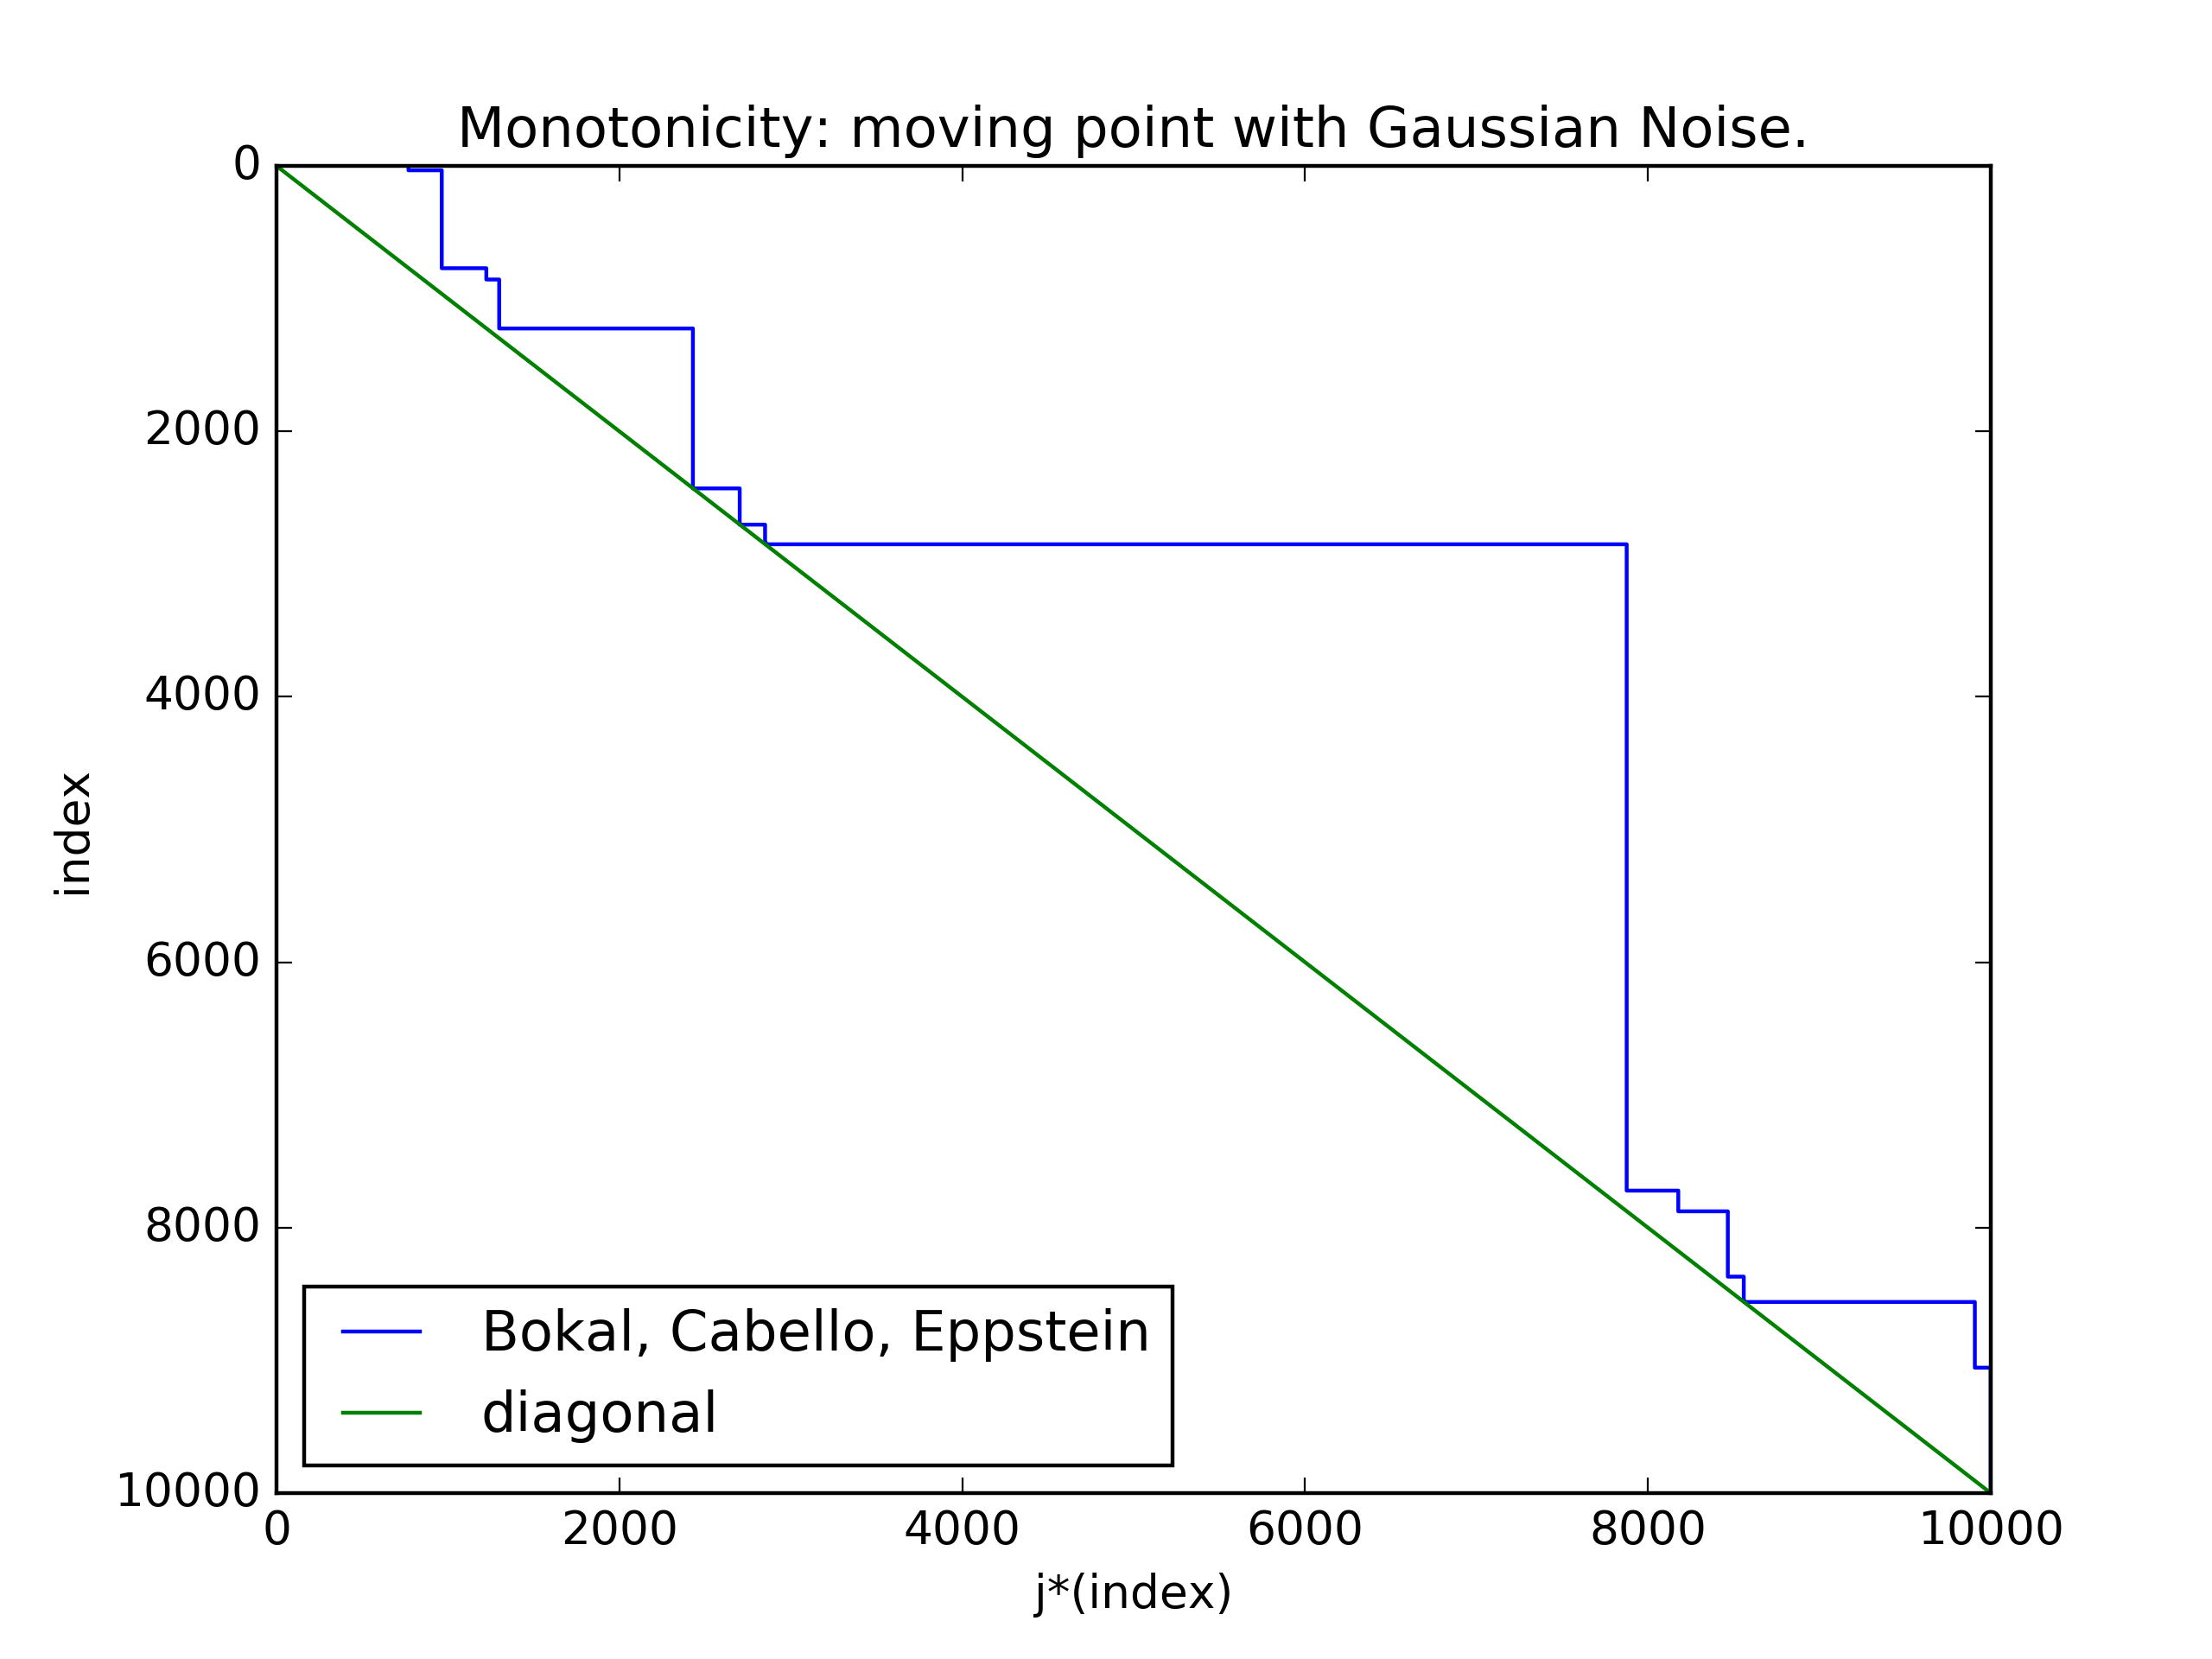
\includegraphics[height=8cm]{../plots/monotonicity_moving_gaussian}
  \caption{Monotonicity algorithm results for moving point with Gaussian noise.}
  \label{fig:monotonicity_demo}
\end{figure}

First let's look at the monotonicity resutls. Here we use the following dataset.

We have a point moving along $x$ axis in the positive direction with speed 1 (i.e. 1 per index), we add Gaussian noise to this point to make the problem interseting. In Figure \ref{fig:monotonicity_demo} you can see results for noise with standard deviations $\sigma_y = 0.05, \sigma_y = 1$. After we generate the dataset, we run Bokal et. al algorithm on the dataset and the answer boundarries of the matrix $A$ that indicates if for points in range $[i, j]$ exists a common direction that has positive dot product with each of the displacements.

Figure \ref{fig:monotonicity_comparison} shows runtime differences in millliseonds between Naive algorithm and algorithm we presented from Bokal et al.
\begin{figure}[!ht]
  \centering
  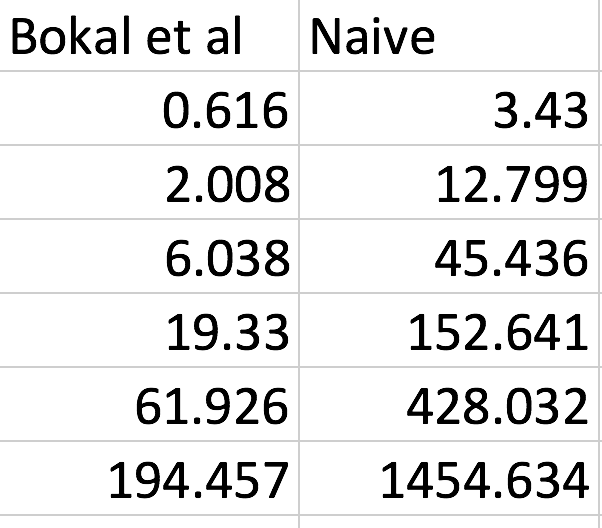
\includegraphics[height=5cm]{../plots/monotonicity_comparison}
  \caption{Runtimes (in millseconds) of Naive and Bokal et. al}
  \label{fig:monotonicity_comparison}
\end{figure}

\subsection{Diameter}

Now the dataset is a random walk starting at the origin. At each step we uniform randomly pick a direction, and move 0.3 distance in that direction. We keep doing this until we have enough points for an experiment.

TODO: Describe Naive algorithm which is a $O(n^2)$ algorithm.

\begin{figure}[!h]
  \centering
  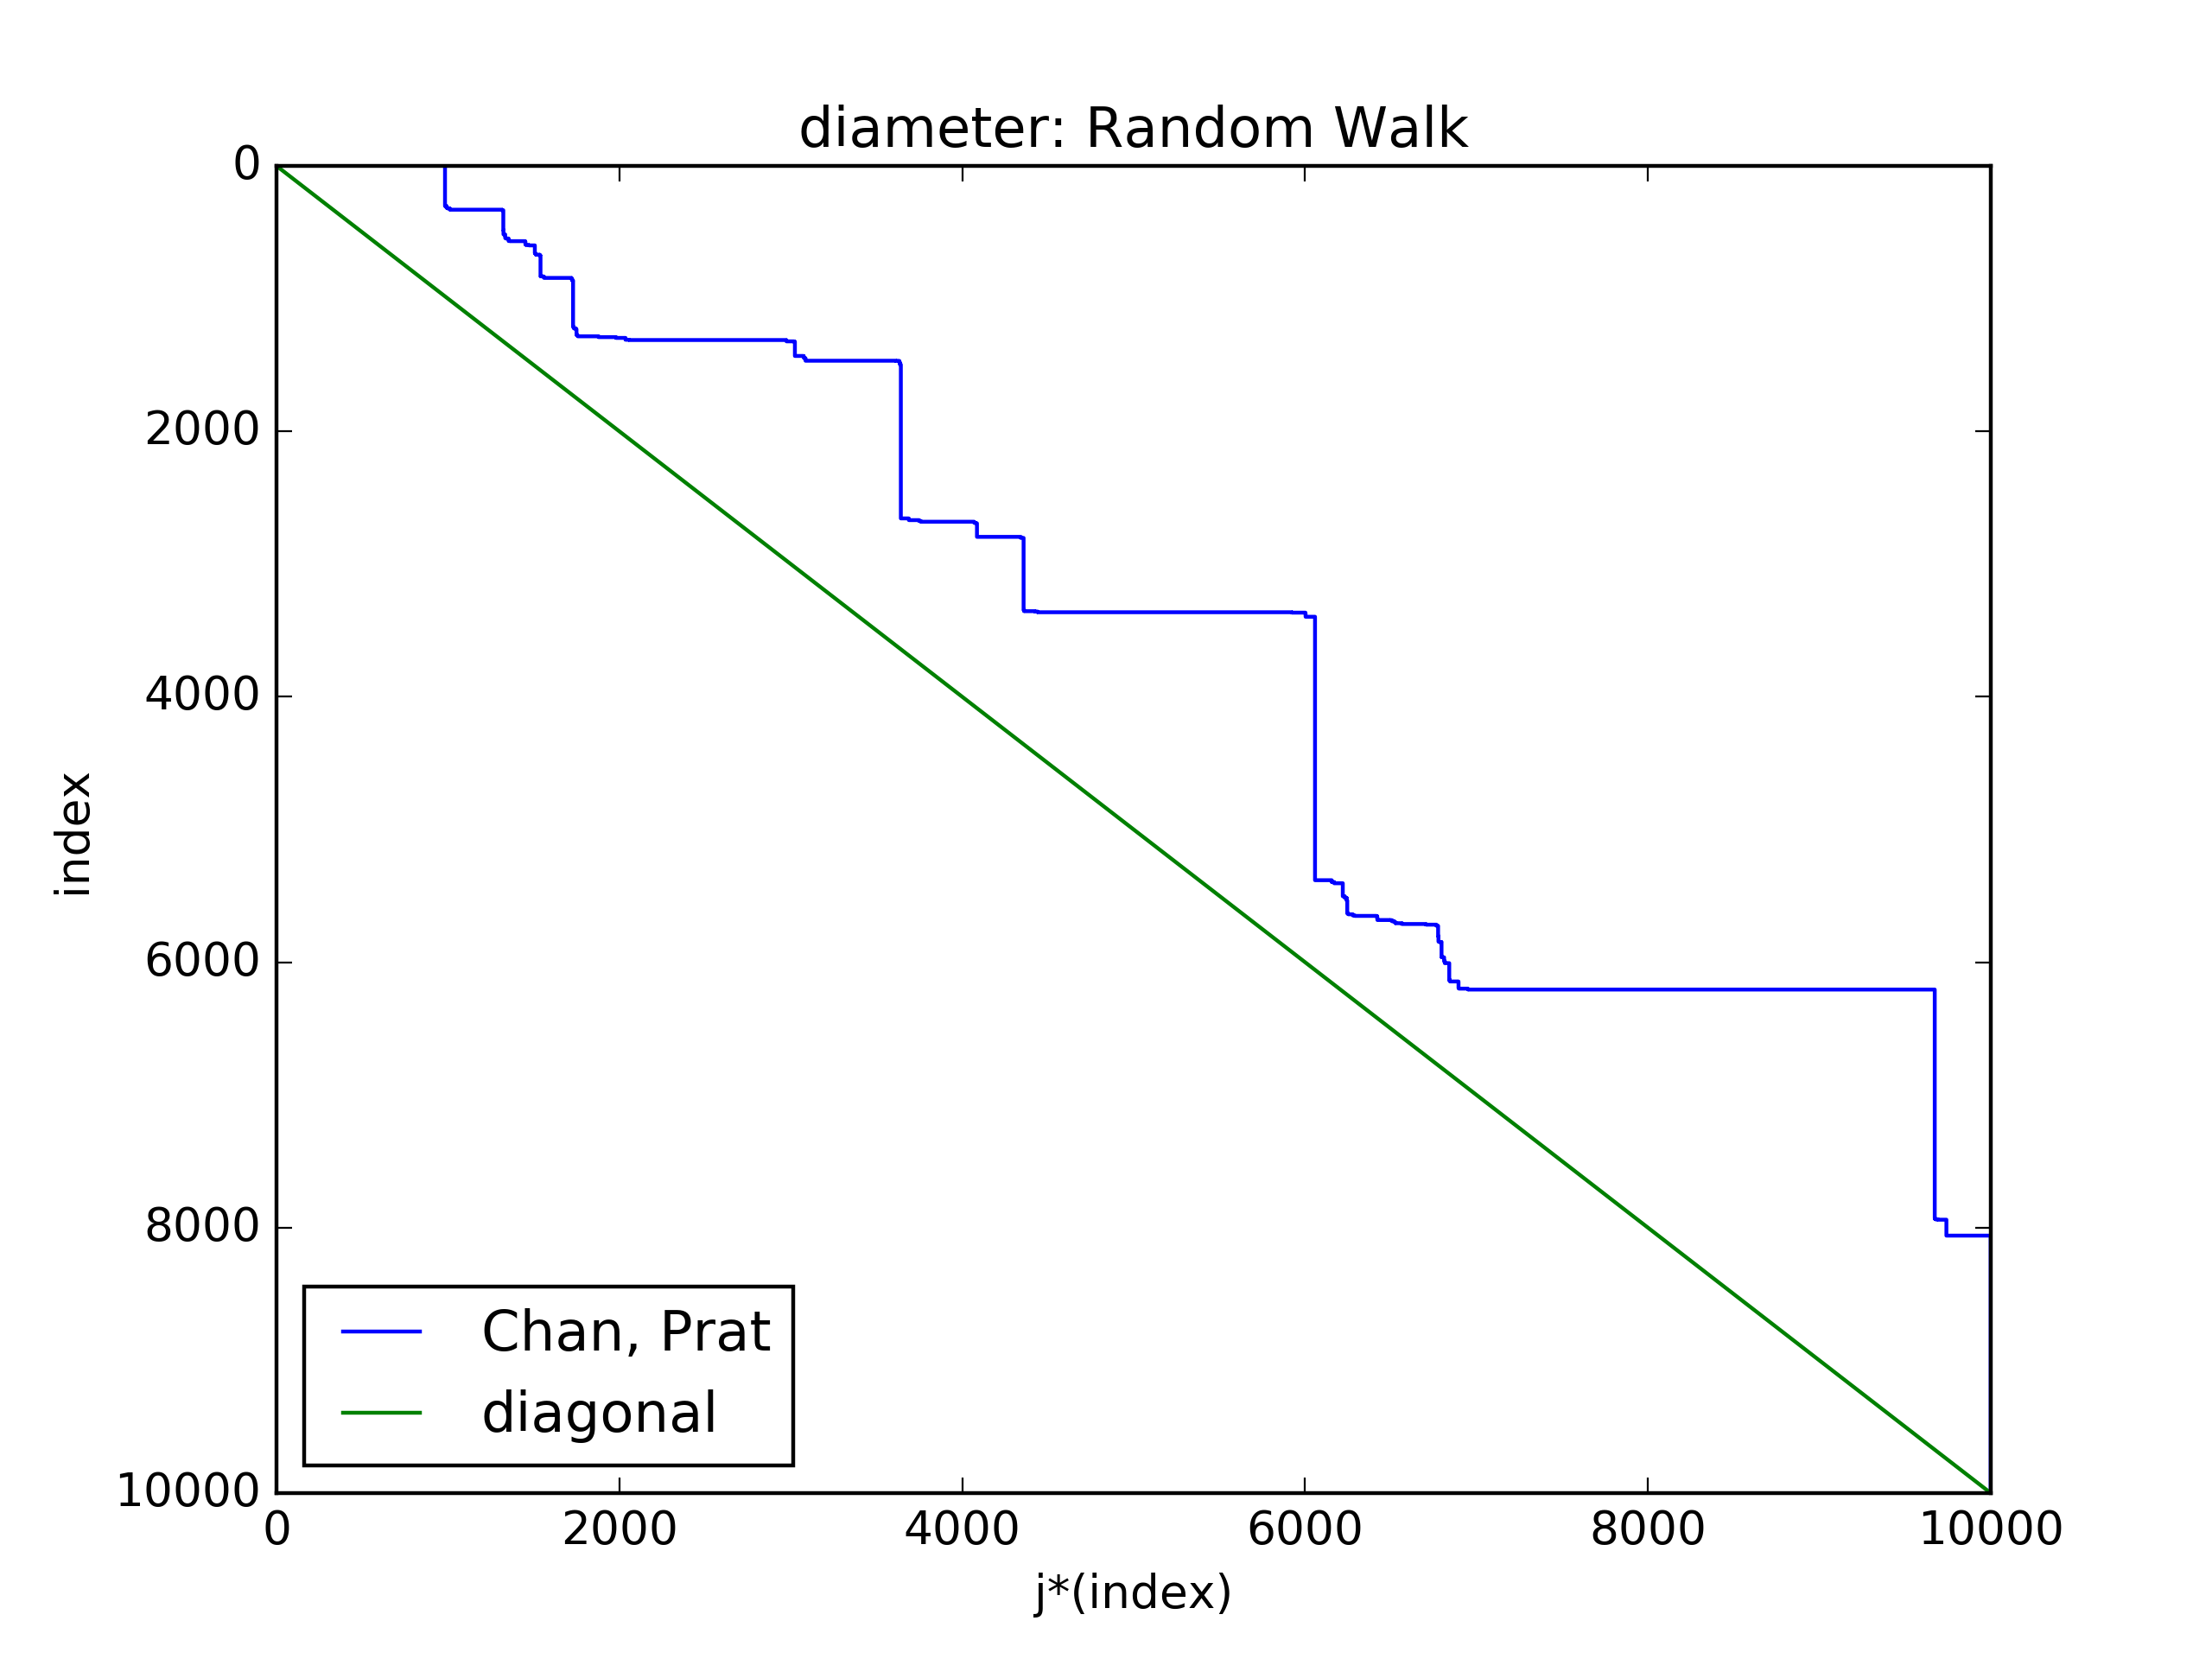
\includegraphics[height=8cm]{../plots/diameter_random_walk}
  \caption{Caption...}
  \label{fig:diameter_demo}
\end{figure}

Figure \ref{fig:diameter_demo} shows boundaries of points that satisfy all points in range $[i, j]$ fall into some circle with radius 1.

Figure \ref{fig:diameter_comparison} will show results comparing runtimes of Naive algorithm with algorithm we presented from Bokal et al.
\begin{figure}[!ht]
  \centering
  
\includegraphics[height=5cm]{../plots/diameter_comparison}
  \caption{Runtimes (in millseconds) of Naive and Chan, Prat [Similar to Figure \ref{fig:monotonicity_comparison}}
  \label{fig:diameter_comparison}
\end{figure}

\section{Conclusion}
It was really challanging to do an implementation project in computational geometry, some sentences in the papers take 100+ lines of code to implement. Thus, for small datasets, added complexity is not worth the speedup gained by the algorithm.

This was a great project otherwise, we've implemented couple of algorithms that we have seen during the lecture - sweep line, range tree, intersection of convex polygons using envelopes. Also couple that we had not found in Bokal et al and Chan, Prat.

\bibliographystyle{unsrt}
\bibliography{papers}
\end{document}
